\chapter{\textit{Mockup} da aplicação \textit{mobile}}
\label{Mockup}

Nas figuras \ref{mock1} e \ref{mock2} são apresentados os \textit{mockups} da aplicação \textit{mobile} prevista. 


\begin{figure}[h]
	\centering
	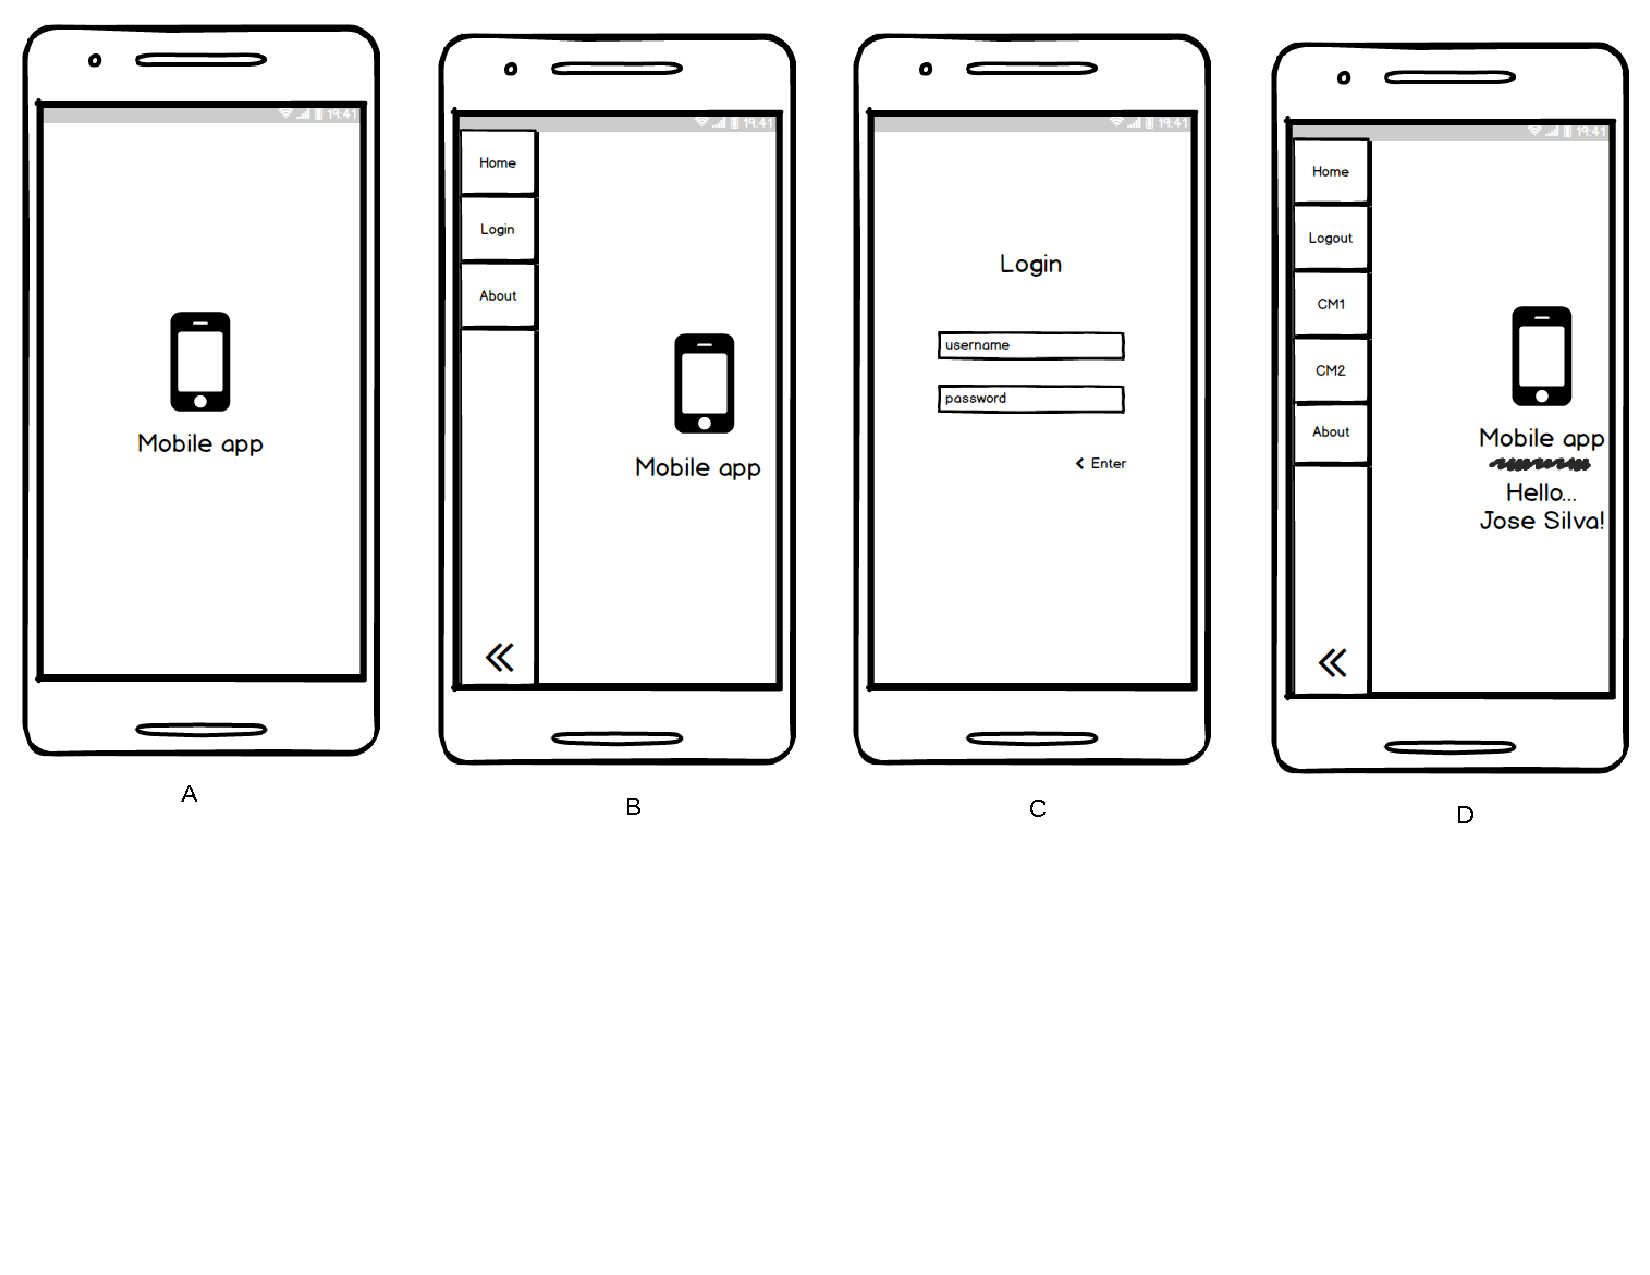
\includegraphics[width=\linewidth]{esquemas/mockup/1.pdf}
	\caption{Mockup da aplicação mobile}
	\label{mock1}
\end{figure}

\begin{itemize}
	\item \textbf{A}: 
	\item \textbf{B}: com sidebar 
	\item \textbf{C}: 
	\item \textbf{D}:
\end{itemize}


\newpage


\begin{figure}[h]
	\centering
	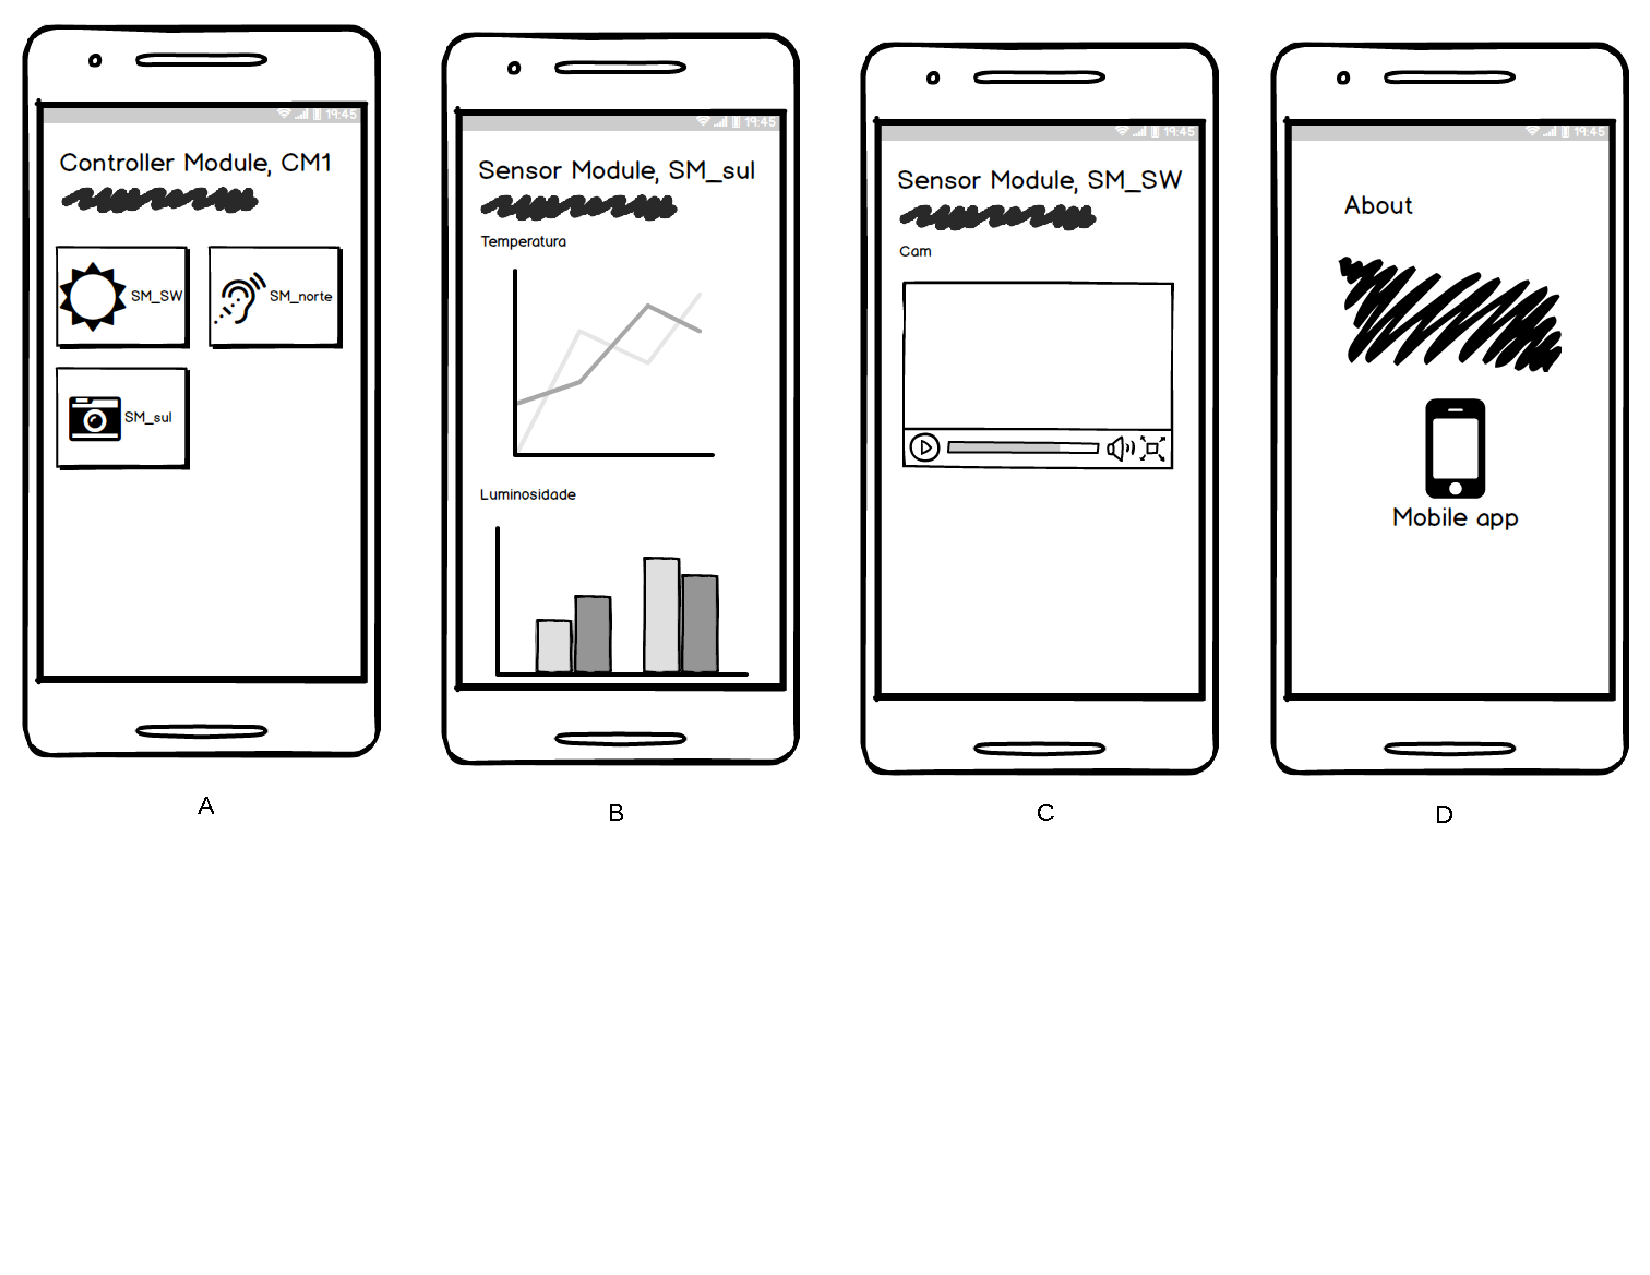
\includegraphics[width=\linewidth]{esquemas/mockup/2.pdf}
	\caption{Mockup da aplicação mobile (continuação)}
	\label{mock2}
\end{figure}

\begin{itemize}
	\item \textbf{A}: 
	\item \textbf{B}: 
	\item \textbf{C}:
	\item \textbf{D}:
\end{itemize}